% !TEX root = ../main.tex
\chapter{Diagnosis Algorithm} \label{ch:diagnosis}
In this chapter will be outlined the diagnosis algorithm\cite{semantic_diagnoser} developed by IBM Research with the collaboration of Michael Maghella, a fellow student at Università degli Studi di Brescia. This algorithm is based on a novel reputation-based approach that makes use of the informations available in the semantic graph to identify cause-effect relationships and use these relationships to isolate relevant causes basing the diagnosis on the timeseries data.
\section{General description}
The diagnosis activity is comprised of three main step:
\begin{itemize}
  \item fault detection, that is the discovery of the fault. A diagnoser needs to be able to tell apart the normal behaviours from faulty ones. This is done, in this approach, through the rules discovered while learning the normal behaviour of a building (see \autoref{subsec:learn_behaviour}). Whenever a fault is detected the diagnosis process ought to start.
  \item fault isolation, that is the discovery of the causes of the fault. It is a key step for enabling a precise diagnosis of the problem. In this approach informations derived from the semantic graph are used to narrow down the set of possible faults to the most relevant ones.
  \item fault identification, that is to determine with some confidence which are the actual causes of a fault among all the possible causes. The proposed diagnoser implements a voting scheme to identify these causes.
\end{itemize}
While explaining the diagnosis approach, it will be used the same model presented in \autoref{ch:model} ( \autoref{fig:ex_building_full}), that will be represented in a compact notation shown in \autoref{fig:simple_model}, where every component is an instance of a concept with the same name (internalized representation).
\begin{figure}
  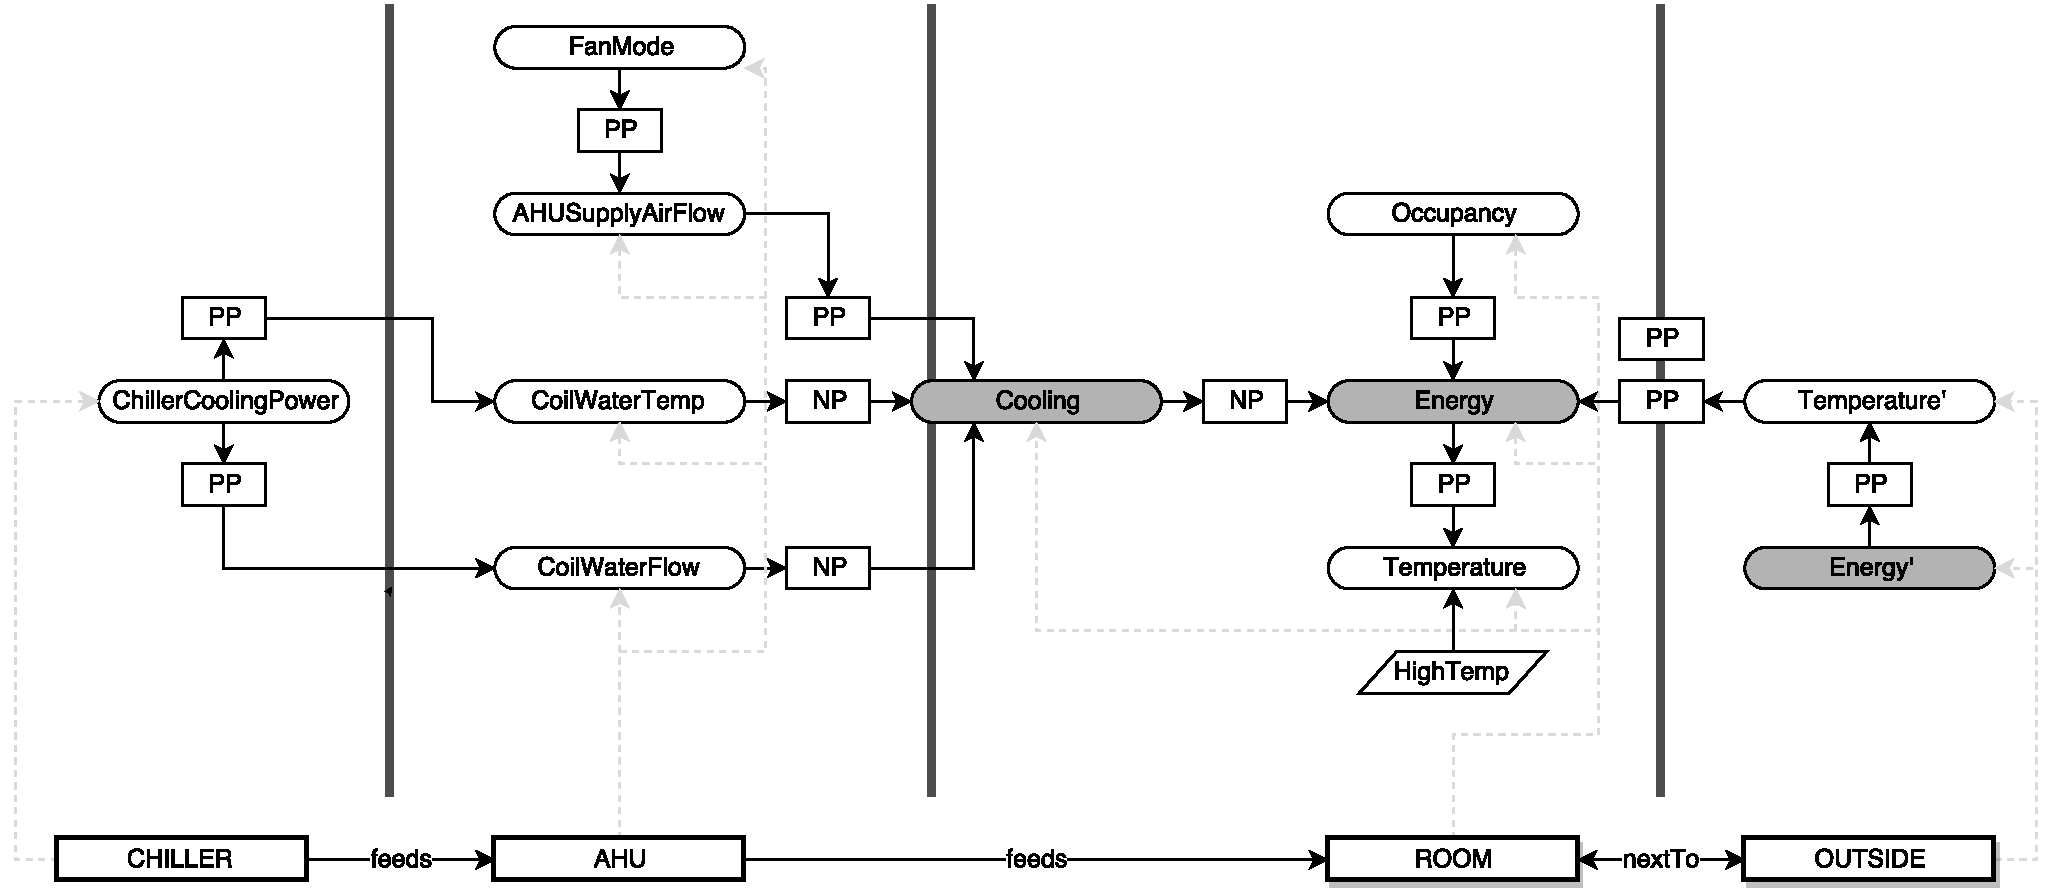
\includegraphics[width=\textwidth]{simple_diagnosis_ex.pdf}
  \caption{Internalized model of the example building}
  \label{fig:simple_model}
\end{figure}
The diagnoser is run every time an anomaly is detected in the timeseries. An anomaly is intended as a deviation from the normal behaviour clearly detectable by some preset upper and lower bounds, therefore an anomaly can be classified as high or low.
It is assumed that an anomaly is symptom of some kind of fault in the system. The algorithm starts, as soon as the anomaly is detected, by identifying the semantic type of the anomaly and the potential causes in the graph. It proceeds computing the voting vector and, eventually, it is recursively executed for all those properties that get a voting score equals or greater then one. When no other causes with a high score are left, the algorithm terminates and produces a list of the detected causes along with the name of the faulty property, the semantic type of the fault and the estimatation, expressed in percentage, of the responsability of that cause towards the diagnosed anomaly.
